\documentclass[11pt,oneside,a4paper]{article}

\usepackage{custom}

\newcommand{\question}
{
\addtocounter{section}{1}
\section*{Question \thesection}
}

\newcommand{\myX}[2]{x_{#1,\text{#2}}}
\newcommand{\xSemaine}[1]{\myX{s}{#1}}
\newcommand{\xn}{\xSemaine{n}}
\newcommand{\xsup}{\xSemaine{sup}}
\newcommand{\xstock}{\xSemaine{stock}}
\newcommand{\xretard}{\xSemaine{retard}}
\newcommand{\xsst}{\xSemaine{sst}}

\newcommand{\myN}[2]{n_{#1,\text{#2}}}
\newcommand{\nSemaine}[1]{\myN{s}{#1}}
\newcommand{\nouv}{\nSemaine{ouv}}
\newcommand{\nemb}{\nSemaine{emb}}
\newcommand{\nlic}{\nSemaine{lic}}

\newcommand{\texttts}[1]{{\small\texttt{#1}}}

\title{Projet d'optimisation}
\author{Groupe 1}
\date{\today}

\begin{document}

%=====================================
%=========PAGE DE GARDE==============
%=====================================

\begin{titlepage}
      \center
      
      LINMA 1702 Mod\`{e}les et m\'{e}thodes d'optimisation \hfill Projet -- 2015\\ 
      \vspace{0.7cm}
      {\LARGE \textsc{Universit\'e Catholique de Louvain}}\\
      {\large \textsc{\'Ecole Polytechnique de Louvain}}\\

      
      \vspace{0.7cm}
      \hrulefill
      \\
      \vspace{0.7cm}
      {\huge \textbf{Planification de la production}} \\ 
      \vspace{0.7cm}
      {\huge \textbf{d'une ligne d'assemblage de smartphones}} \\
      \vspace{0.5cm}
      \hrulefill
      \\
      \vspace{0.3cm}
      
  \begin{center}
      \includegraphics*[height=0.4\textheight]{img/cover_photo.jpg}
      \end{center}      
      
      \vspace{0.2cm}      
      
	{ \Large
	\begin{center}
	\textbf{Groupe 1}
	\end{center}
	}
	
		
	\vspace{0.2cm}	
	
      \begin{tabular}{lc}
     John \textsc{de Wasseige} & (???-1300) \\
	Antoine \textsc{Legat} & (4776-1300) \\
	Quentin \textsc{Lété} & (????-1300) \\
      \end{tabular}
      
      \vfill
      




%----------------------------------------------------------------------------------------
%	DATE SECTION
%----------------------------------------------------------------------------------------

\vfill
{\normalsize 2014 - 2015}\\

%----------------------------------------------------------------------------------------
%	LOGO SECTION
%----------------------------------------------------------------------------------------
  
\includegraphics[height = 0.07\textheight]{img/ucl.png} \hfill
  
\includegraphics[height = 0.07\textheight]{img/epl.jpg}
%----------------------------------------------------------------------------------------

\end{titlepage}

\part{Modélisation et implémentation \\de la ligne d'assemblage simple}

\question %1
\emph{Donnez une formulation linéaire (continue, sans variables entières)
du problème de la planification de la ligne d'assemblage à personnel constant.
Décrivez successivement variables, contraintes et fonction objectif.
A ce stade, le fait de ne pas imposer l'intégralité des variables
vous parait-il problématique ?}

\subsection*{Variables}
Le tableau~\ref{tab:variablesQuestion1} contient les différentes variables $x_{s,\lambda}$
qui correspondent au nombre de smartphones pour chaque semaine $s$
avec la caractéristique $\lambda$.

\begin{table}[h]
  \begin{center}
  \begin{tabular}{|l|l|}
    \hline
    Variable & Caractéristiques des smartphones \\
    \hline
    \hline
    $\xn$ & Produits au \emph{salaire normal}. \\
    \hline
    $\xsup$ & Produits pendant les \emph{heures supplémentaires}. \\
    \hline
    $\xstock$ & Conservés en \emph{stock}. \\
    \hline
    $\xretard$ & Vendus une semaine en \emph{retard}. \\
    \hline
    $\xsst$ & Sous-traités. \\
    \hline
  \end{tabular}
  \caption{Variables de la modélisation de la ligne d'assemblage simple.}
  \label{tab:variablesQuestion1}
  \end{center}
\end{table}

\subsection*{Contraintes}
Voici les contraintes du problème de la planification
de la ligne d’assemblage à personnel constant.
On pose que $\Delta x_{s,\lambda} = x_{s,\lambda} - x_{s-1,\lambda}$.
Voici les contraintes du problème de la planification 
de la ligne d’assemblage à personnel constant, $s$ étant un naturel allant de $1$ à $T$.
% J'ai retiré
%  \myX{0}{n}&= 0 \\
% \myX{0}{sup}&= 0 \\
% \myX{0}{sst}&= 0 \\
% Puisque s va de 1 à T
\begin{align*}
  \Delta\xstock + \texttts{demande}(s) &= \xn + \xsup
   + \xsst + \Delta\xretard &\forall s \\
  \myX{T}{stock} &= \texttts{stock\_initial} \\
  \myX{T}{retard}&= 0 \\
  \myX{s-1}{retard} + \Delta\xstock &\leq \xn + \xsup + \xsst \text{\footnotemark} &\forall s \\
  \xn &\leq 35\cdot \texttts{nb\_ouvriers}/ d_{a,h}
  &\forall s \\
  \xsup &\leq \texttts{nb\_max\_heure\_sup}\cdot\texttts{nb\_ouvriers}/ d_{a,h}
  &\forall s \\
  \xsst &\leq \texttts{nb\_max\_sous\_traitant} &\forall s \\
  x_{s,\lambda} &\geq 0 &\forall s,\lambda \\
\end{align*}
\footnotetext{Pour limiter les retards à une seule semaine.}

\subsection*{Fonction objectif}
\[ \text{minimiser } \text{coût}_\text{tot} = \sum_{s=1}^{T} \text{coût}(s) \]

où coût$(s)$ est le coût pour la semaine $s$ et vaut
\[
  c_m\, \xn + (c_m + d_{a,h} \, c_{hs})\, \xsup
  + c_s\, \xstock + c_r\, \xretard + c_{sst}\, \xsst.
\]

Le tableau~\ref{tab:constantesQuestion1} contient les abréviations
des constantes utilisées.
\begin{table}[h]
  \begin{center}
  \begin{tabular}{|l|l|}
    \hline
    Paramètre & Constante représentée \\
    \hline
    \hline
    $c_m$ & \texttt{cout\_materiaux} \\
    \hline
    $c_{hs}$ & \texttt{cout\_heure\_sup} \\
    \hline
    $c_s$ & \texttt{cout\_stockage} \\
    \hline
    $c_r$ & \texttt{cout\_retard} \\
    \hline
    $c_{sst}$ & \texttt{cout\_sous\_traitant} \\
    \hline
    $d_{a,h}$ & \texttt{duree\_assemblage}/60, [heures] \\
    \hline
  \end{tabular}
  \caption{Constantes de la modélisation de la ligne d'assemblage simple.}
  \label{tab:constantesQuestion1}
  \end{center}
\end{table}

On remarquera que le terme associé au coût des heures normales des ouvriers
a été omis dans la fonction objectif puisqu'il n'est pas nécessaire.
En effet, les ouvriers ne sont pas payés en fonction du nombre
d'heures qu'ils travaillent réellement mais bien à la semaine et
donc pour un nombre d'heures constant.
Ceci correspond au terme $35\cdot\texttt{cout\_horaire}\cdot
\texttt{nb\_ouvriers}$ qu'il est impossible de minimiser.
Cela n'aura donc pas d'impact sur notre solution,
il faudra seulement modifier le coût total de la manière suivante
\[ \text{coût}_\text{tot} \leftarrow \text{coût}_\text{tot} + T \cdot 35 \cdot\texttt{cout\_horaire}\cdot
\texttt{nb\_ouvriers} \]

A ce stade, le fait de ne pas imposer l'intégralité des variables
parait problématique dans le sens où les solutions ne sont pas 
garanties d'être entières. Ce qui n'est pas envisageable 
vu que celles-ci représentent des quantités de smartphones.
Par exemple, il est possible que
$\xn$ ne soit pas entier si $1/d_{a,h}$ ne l'est pas.

\question %2
\emph{Démontrez que, sous certaines hypothèses raisonnables, 
il est possible de garantir que votre modèle linéaire continu admette toujours
une solution entière, c'est-à-dire ne comportant que des quantités produites
entières chaque semaine. 
L'une de ces hypothèses est l'intégralité de la demande chaque semaine ; 
quelles sont les autres ?}

Il est possible de garantir que notre modèle linéaire continu
admette toujours une solution entière sous certaines hypothèses.
Une première hypothèse est que tous les éléments du 
vecteur \texttt{demande} soient entiers.
Il faut également que les constantes \texttt{stock\_initial}, \texttt{nb\_max\_sous\_traitant} et 
\texttt{nb\_ouvriers} soient entières bien sûr, sinon cela n'aurait d'ailleurs pas de sens physique.
Mais il est également nécessaire que \texttt{nb\_max\_heure\_sup} soit entier et que $d_{a,h}$ soit multiple de $35\cdot \texttts{nb\_ouvriers}$ et de $\texttts{nb\_max\_heure\_sup}\cdot\texttts{nb\_ouvriers}$, ce qui implique qu'il soit aussi entier.
Notons enfin que nous supposons ces constantes positives, sans quoi notre modèle produirait des résultats aberrants,
voire pas de résultat du tout.

\subsubsection*{Preuve}
Pour le prouver, nous allons reformuler notre problème sous la forme d'un problème de flot de coût minimum.
Soit le graphe orienté $G(V,E)$, 
où $V$ représente l'ensemble des noeuds et $E$ l'ensemble des arêtes.
Il est utile à ce stade de s'aider d'un schéma représentant le graphe. 
Celui-ci est repris à la figure~\ref{fig:schemaFlot}.
$V$ compte un noeud pour chaque semaine et un noeud initial.
On a donc $V := {0, 1, 2, ..., T}$
où $0$ est le noeud initial et $s$ est le noeud de la semaine $s$.
Définissons maintenant les arêtes de notre graphe.
Pour le noeud $0$, on définit\footnote{Notations : $V^{-}(s)$ désigne l'ensemble des noeuds dont l'arête ``rentre'' dans le noeud s, à l'inverse $V^{+}(s)$ désigne les ``sortants''.}

\begin{figure}[h]
	\centering
		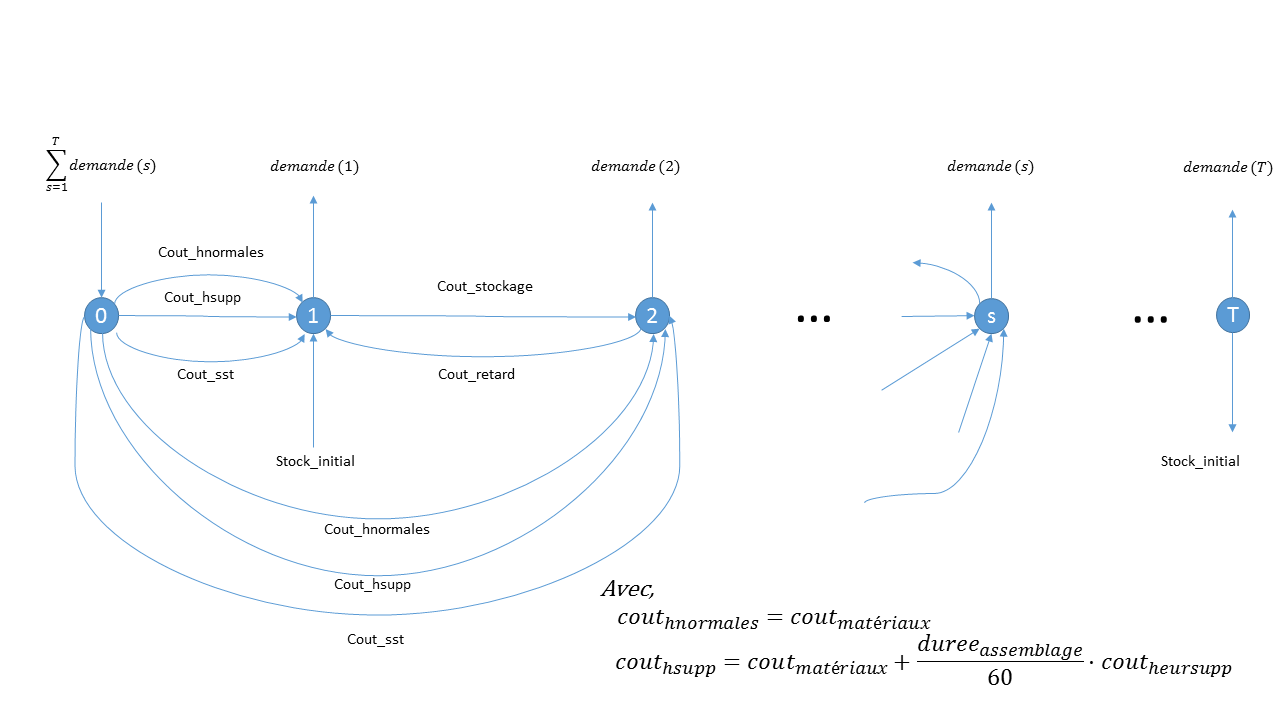
\includegraphics[scale = 0.7, angle = 90]{img/Schema_flot.png}
	\caption{Schéma représentant le graphe utilisé pour définir 
  le problème de flot de coût minimal.}
	\label{fig:schemaFlot}
\end{figure}

\[ V^{+}(0) = \{s_1, s_2, s_3 \quad \forall s \ne 0\} \]
avec
\[ \{(0, s_1), (0, s_2), (0, s_3)\} \in E \quad \forall s. \]
$s_1$, $s_2$, $s_3$ représentent les différentes manières de produire les smartphones, c'est-à-dire les ouvriers au salaire normal, les ouvriers au salaire des heures supplémentaires et la sous-traitance.
Il y a donc trois arcs entre les noeuds $0$ et $s$.
Pour le noeud initial,
\[ V^{-}(0) = \emptyset \]
Définissons ensuite les arêtes des noeuds correspondants aux semaines
\[ V^{+}(s) = \{s+1\} \qquad \forall s \ne 0 \]
avec 
\[ \{(s, s+1)\} \in E \qquad \forall s \ne 0, T \]
Et,
\[ V^{-}(s) = \{0, s-1\} \qquad \forall s \ne 0 \]
avec
\[ \{(s-1, s)\} \in E \qquad \forall s \ne 0, 1 \]
Nous devons encore définir les termes sources pour chaque noeud ainsi que les capacités maximales pour chaque arc.
Soit
\[ b_s = - \texttts{demande}(s) \qquad s \in V \backslash \{0\} \]
Et 
\[ b_0 = \sum_{s=1}^{T} \texttts{demande}(s) \]  
On a aussi
\[ b_1 = \texttts{stock\_initial} \]
Et
\[ b_T = - \texttts{stock\_initial} \]
Soient $h_{ij}$ avec $(i, j) \in E$ les capacités maximales dans l'arc $(i, j)$.
On a $\, \forall s \ne 0$ 
\begin{align*}
  h_{0, s_1} &= 35\cdot \texttts{nb\_ouvriers}/ d_{a,h} \\
  h_{0, s_2} &= \texttts{nb\_max\_heure\_sup}\cdot\texttts{nb\_ouvriers}/ d_{a,h} \\
  h_{0, s_3} &= \texttts{nb\_max\_sous\_traitant} 
\end{align*}
Le graphe maintenant défini, 
on peut définir le problème de minimisation suivant :
\paragraph{Variables}
Soit $x_{ij}$ le flot dans l'arc $(i, j)$.
\paragraph{Objectif}
Le coût total est minimisé.
\[ \sum_{(i, j) \in E} c_{ij} x_{ij} \]
\paragraph{Equations} Le flot est conservé en chaque noeud
\[ \sum_{k \in V^{+}(i)} x_{ik} - \sum_{k \in V^{-}(i)} x_{ki} 
  = b_i \qquad i \in V
\]
Les capacités maximales ne sont pas dépassées
\[ 0 \leq x_{ij} \leq h_{ij} \qquad (i, j) \in E \]

On peut maintenant utiliser le théorème suivant pour conclure que, si nos hypothèses sont vérifiées, notre problème admettra au moins une solution entière.
\paragraph{Théorème}
Si les demandes $b_i$ et les capacités $h_{ij}$ 
d'un problème de flot de coût minimum sont entières alors il existe une solution optimale entière.
\footnote{En regardant de plus près la démonstration de ce résultat,
on note également que chaque sommet est entier. 
Cependant, ce théorème ne nous dit \emph{pas} que \emph{toutes} 
les solutions optimales sont entières.}

Nous devons donc imposer que \texttt{stock\_initial} et tous les éléments du vecteur \texttt{demande} soient entiers afin que tous les $b_i$ le soient. Pour trouver les hypothèses relatives aux $h_{ij}$, nous procédons de la manière suivante. \texttt{nb\_ouvriers} doit être entier, sans quoi cela n'a pas de sens physique. Or, pour que $h_{0, s_1}$ soit entier, $35\cdot \texttts{nb\_ouvriers}$ doit être divisible par $d_{a,h}$, ce qui équivaut à dire que $d_{a,h}$ est multiple de $35\cdot \texttts{nb\_ouvriers}$. On en conclut aussi que $d_{a,h}$ est entier. Nous raisonnons de la même manière pour $h_{0, s_2}$ et trouvons que $d_{a,h}$ doit également être multiple de $\texttts{nb\_max\_heure\_sup}\cdot\texttts{nb\_ouvriers}$. On en déduit que \texttt{nb\_max\_heure\_sup} est lui aussi entier. Enfin, \texttt{nb\_max\_sous\_traitant} doit lui aussi être entier.

On note que les deux hypthèses ``$d_{a,h}$ est multiple de \dots'' seront satisfaites si \texttt{nb\_ouvriers} est multiple de $d_{a,h}$ (ou même encore plus simplement si $1/d_{a,h}$ est entier). Mais il faut être attentif au fait que cette condition, bien que suffisante, n'est \emph{pas nécessaire}. En effet, on peut considérer l'exemple où $\texttts{nb\_ouvriers} = 1$, $d_{a,h}=5$ et $\texttts{nb\_max\_heure\_sup} = 10$. Les hypothèses sont alors remplies sans que \texttt{nb\_ouvriers} ne soit multiple de $d_{a,h}$ (et sans que $1/d_{a,h}$ ne soit entier).
\question %3
\emph{Implémentez sous MATLAB ce modèle linéaire continu,
et calculez la solution correspondant aux données fournies sur icampus
(utilisez la fonction \texttt{linprog}).
Commentez l'allure de la solution obtenue.}

Notre implémentation se trouve dans le fichier \texttt{question3.m}.
Il nous parait important d'expliquer en quelques mots le r\^ole
de la fonction \texttt{kron}.
Celle-ci effectue le produit tensoriel de Kronecker entre deux matrices.
C'est-à-dire que pour \texttt{kron(A,B)},
chaque élément de $A$ multiplie la matrice $B$.
En l'utilisant de manière appropriée avec des matrices nulles et diagonales,
on peut effectuer un remplissage des matrices des contraintes très efficace.

Un exemple d'utilisation de cette fonction pour remplir la matrice
des contraintes se trouve dans l'annexe~\ref{app:kron}.

Les résultats obtenus sont représentés graphiquement
à la figure~\ref{fig:grapheProduction}.
Comme on pouvait s'y attendre, la solution optimale utilise presque chaque
semaine au maximum la ressource la moins chère,
en l'occurence la production par les ouvriers payés au salaire normal.
On observe également que la solution optimale constitue un stock dans la première partie de la planification pour faire face au pic de demande
situé entre les semaines 5 et 8.
La demande est particulièrement importante à la semaine 7,
et on voit que notre stock constitué s'épuise totalement lors de cette semaine.
On commence également à avoir recours au retard.

\begin{figure}[H]
  \begin{center}
    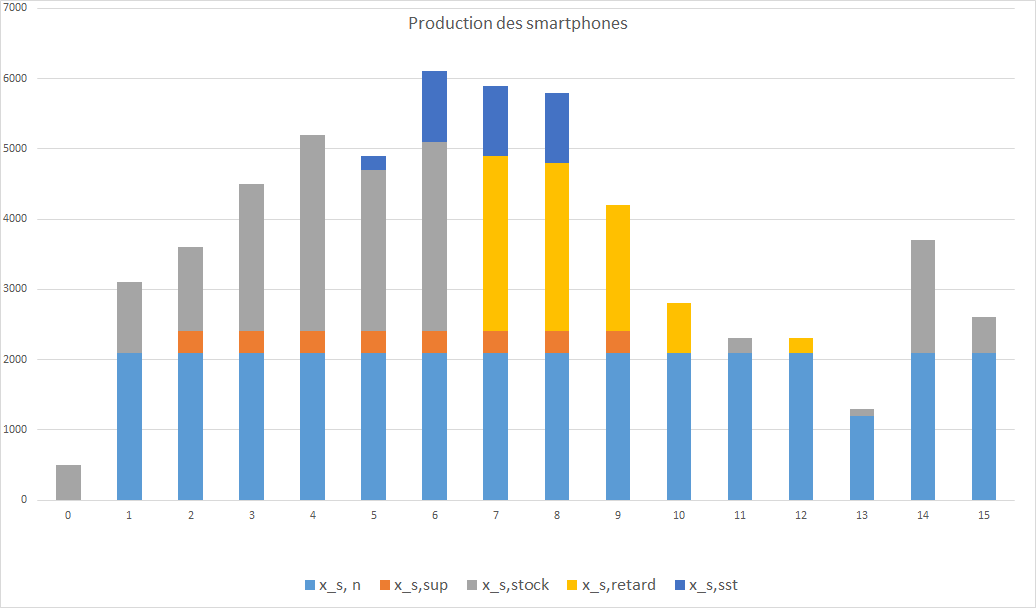
\includegraphics[scale = 0.8]{img/grapheProduction.png}
	  \caption{Répartition du moyen de production des smartphones en fonction des semaines.}
	  \label{fig:grapheProduction}
  \end{center}
\end{figure}

\question %4
\emph{Décrivez une procédure permettant, avec le moins de nouveaux calculs
possibles, d'évaluer les conséquences sur la fonction objectif d’une petite
variation de la demande prévue. Plus précisément, analysez l'effet du
remplacement du vecteur \texttt{demande} 
par le vecteur \texttt{demande + epsilon * delta\textunderscore demande} 
où \texttt{delta\textunderscore demande} est un vecteur de perturbation 
sur la demande, 
et \texttt{epsilon} est un paramètre scalaire dont la valeur est faible.}

Le dual du problème nous permet d'évaluer assez simplement
les conséquences sur la fonction objectif
d'une petite variation de la demande prévue.

En effet, notre problème peut être simplifié sous la forme
\begin{align*} 
	\text{minimiser } c^T x \\
	a_i^T x &= b_i  & i = 1,...,T,...,T+7 \\
  a_i^T x &\leq b_i & i = T+8,...,end \\
	x_j &\geq 0 & \forall j
\end{align*}
On obtient ensuite sa forme duale
\begin{align*} 
	\text{maximiser } b^T y \\
	y_i &\text{ libre} & i = 1,...,T,...,T+7 \\
  y_i &\leq 0 & i = T+8,...,end \\
  A_j^T y &\leq c_j & \forall j
\end{align*}

%Une partie du vecteur $b$ (et plus précisement les $T$ premiers éléments)
%correspond à la demande.
On remarque qu'une perturbation des contraintes dans le problème primal
correspond à une perturbation de la fonction objectif dans le problème dual.
Il nous suffit donc simplement de calculer une solution optimale du dual $y^{*}$
puis d'effectuer le produit scalaire
\[ \Delta z^{*} = (\Delta b)^T y^{*} \]
pour chaque perturbation $\Delta b$ pour conna\^itre l'impact $\Delta z^{*}$
sur le cout.

Ce résultat n'est valable que pour des petites variations de b.
En effet, pour l'obtenir, il faut supposer que l'on connaît un sommet optimal admissible.
Or, en changeant le problème, il n'est pas garanti que ce sommet reste optimal et admissible. 
Plus la perturbation est importante, plus il y a de chances que notre sommet optimal change.

\question %5
\emph{Testez sous MATLAB la procédure du point précédent avec les données
fournies. Comparez ensuite la prédiction obtenue par cette procédure
avec la valeur obtenue en résolvant à nouveau complètement le modèle,
et ce pour un échantillon de valeurs du paramètre \texttt{epsilon} comprises
entre $0$ et $1$ (par exemple \texttt{0:.1:1}). 
Commentez (éventuellement en vous aidant d'un graphique).}

Comparaison À FAIRE.

Notre fonction \texttt{compareDuality.m} permet de prouver l'efficacité
du problème dual lorsqu'on perturbe le vecteur des contraintes.
En effet, si l'on décide d'analyser via le problème primal ce qu'il 
se passe lorsque les contraintes sont modifiées, il est nécessaire de 
résoudre le problème à chaque perturbation 
(plusieurs appels à \texttt{linprog}).
Tandis que pour le problème dual,
il suffit d'effectuer plusieurs combinaisons linéaires de la fonction objectif
avec \emph{une seule} solution $y^{*}$ 
(c'est-à-dire un apppel à \texttt{linprog}).
On retrouve les résultats des tests d'efficacité
sur le graphe de la figure~\ref{fig:efficiencyDual}. 

Cependant, comme expliqué dans la section précédente, ce résultat n'est valable que pour des petites variations des contraintes.
Si \texttt{epsilon} devient trop grand, l'analyse par le primal pourrait diverger de la solution du primal.
C'est ce que nous obtenons en implémentant ces deux méthodes, comme représenté à la figure \ref{fig:responseToPerturbations}

\begin{figure}
  \begin{center}
    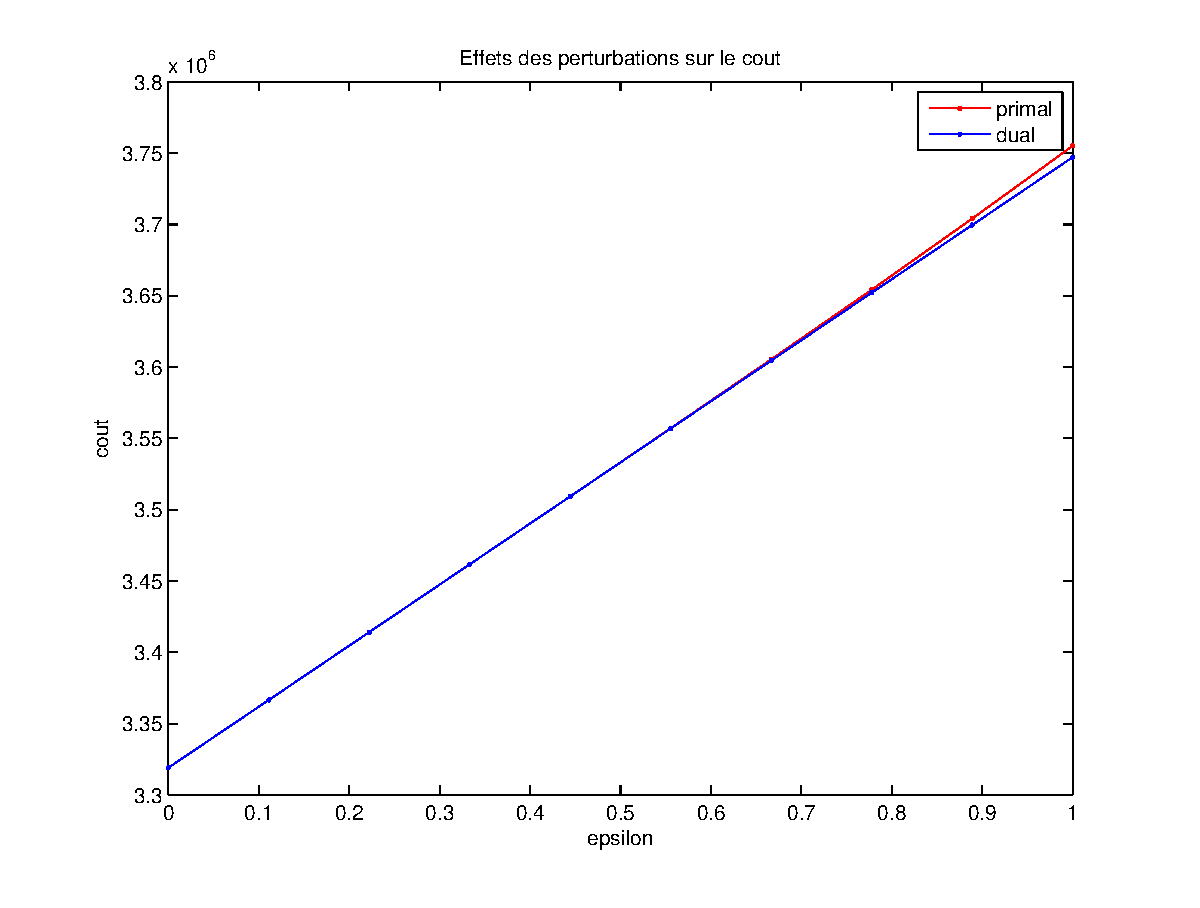
\includegraphics[scale=0.6]{img/responseToPerturbations.eps}
    \caption{Comparaison de la réponse aux perturbations du primal 
    et dual. On remarque que les valeurs restent égales jusqu'à 
    $\epsilon \approx 0.6$.}
    \label{fig:responseToPerturbations}
  \end{center}
\end{figure}

\begin{figure}
  \begin{center}
    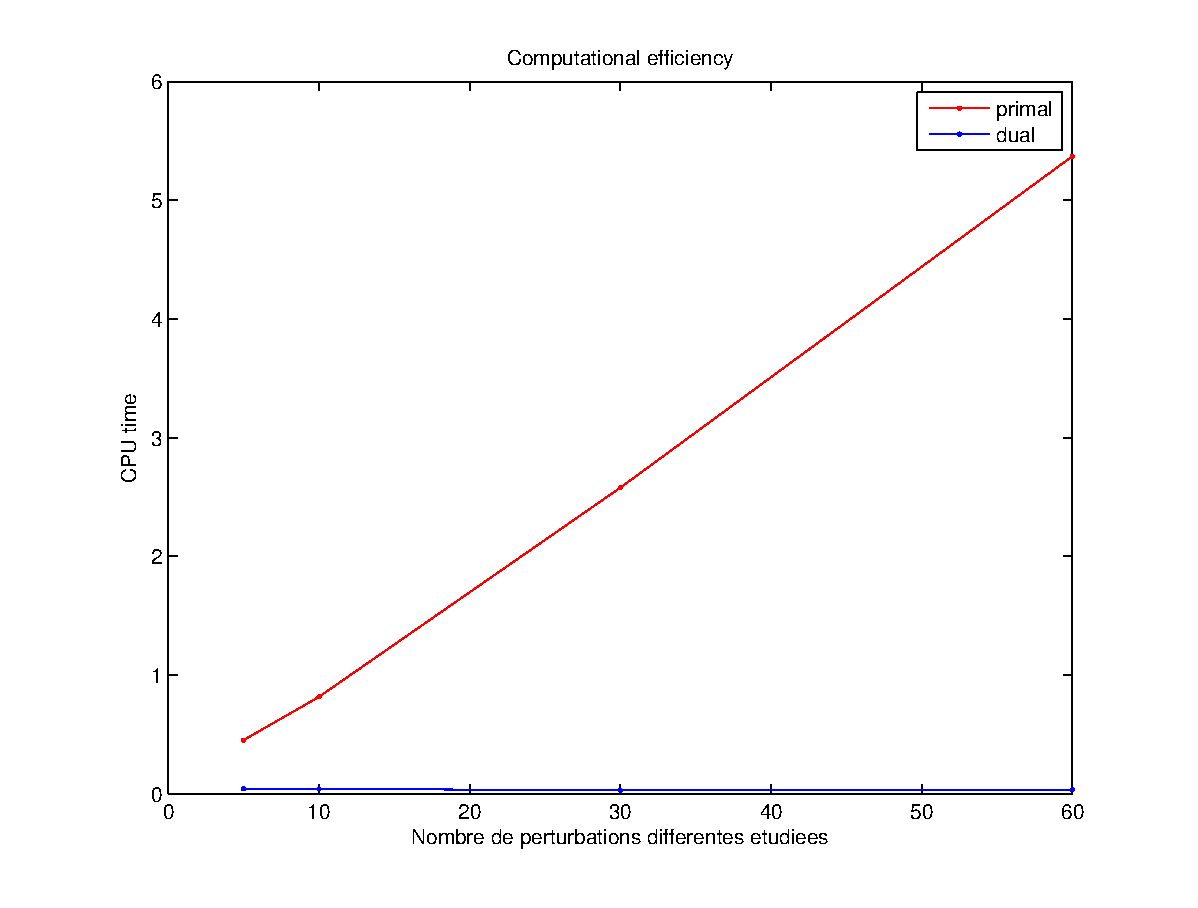
\includegraphics[scale=0.6]{img/efficiencyDual.eps}
    \caption{Comparaison de l'efficacité du primal et dual lors de
    l'analyse de perturbations sur les contraintes.}
    \label{fig:efficiencyDual}
  \end{center}
\end{figure}

\question %6
\emph{Décrivez (sans l'implémenter) l'adaptation qu'il serait nécessaire à
apporter au modèle si le coût de l'heure supplémentaire pris en compte était
variable. Plus concrètement, considérez qu'après la première heure
supplémentaire (facturée au coût horaire \texttt{cout\textunderscore
heure\textunderscore sup} standard), chaque heure supplémentaire
(éventuellement) est facturée à un coût horaire supérieur de $5 \%$
à celui de l'heure supplémentaire précédente.
Est-il toujours possible de formuler (ou reformuler)
le problème sous forme linéaire ? Expliquez.
Et que se passerait-il si le coût horaire des heures supplémentaires \emph{diminuait}
lorsque le nombre d'heures prestées augmente ? Justifiez.}

Si le coût des heures supplémentaires n'est plus constant mais augmente au fur et à mesure de leur utilisation,
le coût de celles-ci dépenderait directement du nombre de smartphones
produits de cette manière.

En effet, on peut réécrire notre fonction objectif comme
\[
  \mbox{minimiser }
  \sum_{s=1}^{T}
  c_m\, \xn + c_m \, \xsup + \mathcal{C}_{hs} (\xsup)
  + c_s\, \xstock + c_r\, \xretard + c_{sst}\, \xsst
\]
avec
\[
  \mathcal{C}_{hs} (\xsup) = \texttts{cout\_heure\_sup} \cdot
  \sum_{i=0}^{\alpha-1}  (1.05)^{i}
\]
Par souci de lisibilité, on a posé
\[ \alpha = \lceil \xsup \, d_{a,h} \rceil \]
$\alpha$ correspond donc au nombre d'heures supplémentaires nécessaires à la production de $\xsup$ smartphones pendant celles-ci, arrondi à l'entier supérieur.

On remarque immédiatement que la fonction $\mathcal{C}_{hs}$
est \emph{non-linéaire} en $\xsup$ puisque $\alpha$ apparaîtra en exposant, et donc $\xsup$ aussi.

De même, si le coût des heures supplémentaires \emph{diminuait}
avec un taux de $0.05$,
on aurait
\[
  \mathcal{C}_{hs} (\xsup) = \texttts{cout\_heure\_sup} \cdot
  \sum_{i=0}^{\alpha-1}  (0.95)^{i}.
\]
Dans les deux cas, il n'est donc plus possible de formuler le problème sous forme linéaire.

\part{Modélisation et implémentation \\de la ligne d'assemblage avec gestion du personnel}

\question %7
\emph{Donnez à présent une formulation linéaire (continue, sans variables
entières) du problème de la planification de la ligne d'assemblage
incluant le gestion du personnel, en vous basant sur le modèle déjà 
construit à la Question 1. Décrivez successivement variables, 
contraintes et fonction objectif.}

Le nombre d'ouvriers n'étant plus constant, nous allons rajouter deux variables
par semaine pour modéliser le problème :
\begin{itemize}
  \item[$\diamond$] $\nemb$ le nombre d'ouvriers embauchés au début de la semaine $s$,
  \item[$\diamond$] $\nlic$ le nombre d'ouvriers licienciés au début de la semaine $s$,
  \item[$\diamond$] $\nouv$ le nombre d'ouvriers au début de la semaine $s$,
  après les embauches et les licenciements.
\end{itemize}

Dans la fonction objectif, il faut maintenant tenir compte du cout de 
ces recrutements et ces licenciements 
ainsi que du coût du salaire des ouvriers, non constant.

En ce qui concerne les contraintes, il faut modifier celles sur 
le nombre de smartphones maximum produits dans l'entreprise. 
Il faut également ajouter les contraintes correspondants 
au nombre d'ouvriers (maximum et minimum).

\subsection*{Fonction objectif}
\begin{align*}
  \mbox{minimiser } 
  \sum_{s=1}^{T} 
  c_m\, \xn &+ (c_m + d_{a,h} \, c_{hs})\, \xsup
  + c_s\, \xstock + c_r\, \xretard + c_{sst}\, \xsst \\
  &+ 35 \, c_{h} \, \nouv 
  + c_{emb} \, \nemb + c_{lic} \, \nlic
\end{align*}

Le tableau~\ref{tab:constantesQuestion7} contient les nouvelles abréviations
des constantes utilisées.
\begin{table}[h]
  \begin{center}
  \begin{tabular}{|l|l|}
    \hline
    Paramètre & Constante représentée \\
    \hline
    \hline
    $c_{h}$ & \texttt{cout\_horaire} \\
    \hline
    $c_{emb}$ & \texttt{cout\_embauche} \\
    \hline
    $c_{lic}$ & \texttt{cout\_licenciement} \\
    \hline
  \end{tabular}
  \caption{Constantes de la modélisation de la ligne d'assemblage
  avec gestion du personnel.}
  \label{tab:constantesQuestion7}
  \end{center}
\end{table}

\subsection*{Contraintes}
Voici les contraintes du problème de la planification 
de la ligne d’assemblage à personnel variable.
\begin{align*}
  \Delta\xstock + \texttts{demande}(s) &= \xn + \xsup 
  + \xretard + \xsst - \myX{s-1}{retard} &\forall s \\
  \Delta\nouv &= \nemb - \nlic &\forall s \\
  \myX{0}{n}&= 0 \\
  \myX{0}{sup}&= 0 \\
  \myX{0}{stock}&= \texttts{stock\_initial} \\
  \myX{0}{retard}&= 0 \\
  \myX{0}{sst}&= 0 \\
  \myN{0}{ouv}&= \texttts{nb\_ouvriers} \\
  \myN{0}{emb}&= 0 \\
  \myN{0}{lic}&= 0 \\
  \myX{T}{stock}&= \texttts{stock\_initial} \\
  \myX{T}{retard}&= 0 \\
  \myX{s-1}{retard} + \Delta\xstock &\leq \xn + \xsup + \xsst &\forall s \\
  \xn &\leq 35\cdot \nouv / d_{a,h}
  &\forall s \\
  \xsup &\leq \texttts{nb\_max\_heure\_sup}\cdot \nouv / d_{a,h}
  &\forall s \\
  \xsst &\leq \texttts{nb\_max\_sous\_traitant} &\forall s \\
  \nouv &\leq \texttts{nb\_max\_ouvriers}  &\forall s \\
  x_s, n_s&\geq 0 &\forall s
\end{align*}

\question %8
\emph{Implémentez sous MATLAB ce modèle linéaire continu,
et calculez la solution correspondant aux données fournies sur icampus.
Commentez l'allure de la solution obtenue, et comparez à la solution du modèle
simplifié. Commentez également l'intégralité des variables de la solution ;
celle-ci présente-t-elle un aspect problématique ?}

\begin{figure}[H]
  \begin{center}
    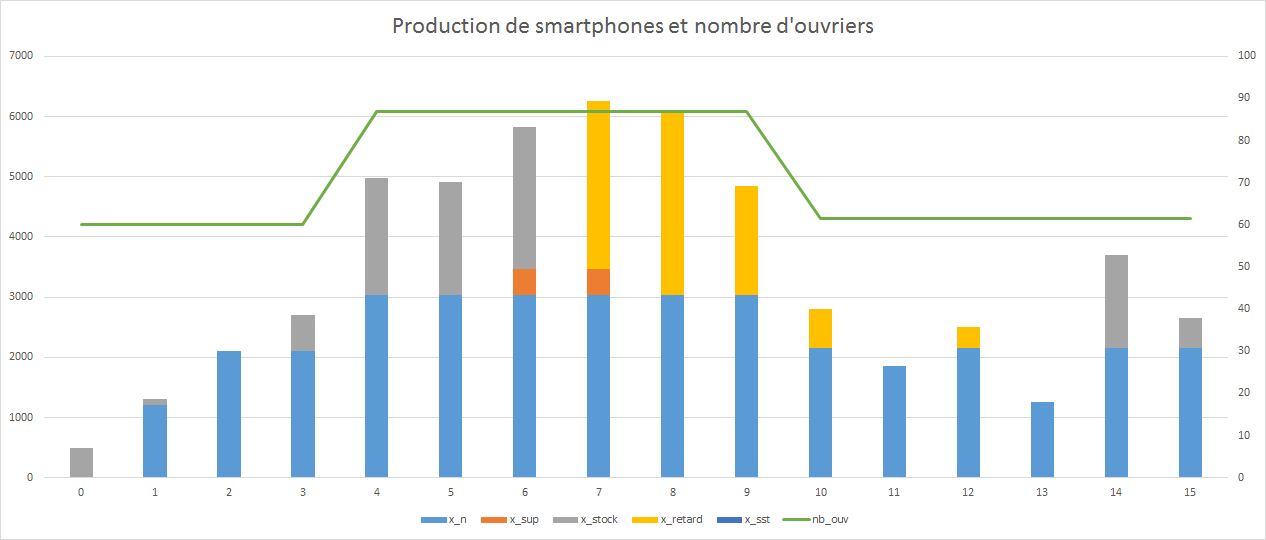
\includegraphics[scale = 0.75]{img/grapheProductionOuvNonInt.png}
	  \caption{Répartition du moyen de production des smartphones en fonction des semaines et évolution du nombre d'ouvriers dans le cas non entier.}
	  \label{fig:grapheProductionOuvNonInt}
  \end{center}
\end{figure}

Les résultats de cette nouvelle implémentation sont présentés à la figure \ref{fig:grapheProductionOuvNonInt}. Les résultats obtenus ne sont plus entiers car le problème ne peut plus être reformulé comme un problème de flot. Ceci est problématique car il serait impossible de réaliser cette production exacte en pratique. Pour les applications, il est plus intéressant de chercher la solution otimale entière. C'est pourquoi nous commenterons l'allure de la solution à la question 9 où nous avons résolu le problème en variables entières. Néanmoins, nous pouvons déjà faire deux remarques à ce stade :
\begin{itemize}
\item Le coût est ici de 3.755.214 unités. En comparaison, le coût obtenu par résolution en variables entières est de 3.755.300 unités. Il y a donc une différence de coût, certes très faible. La nouvelle contrainte appliquée au système, celle de résoudre en variables entières, nous fait perdre en efficacité. 
\item Les résultats du modèle en variables continues sont très semblables à ceux du modèle en variables entières, présentés à la figure \ref{fig:grapheProductionOuv}. La seule différence notable est l'utilisation de retard à la place d'ouvriers payés au salaire des heures supplémentaires lors de la huitième semaine, probablement due à la faible différence de coût entre les deux possibilités.
\end{itemize}
\question %9
\emph{Résolvez à nouveau ce modèle en imposant à présent l'intégralité des
variables pour lesquelles c'est absolument indispensable
(utilisez la fonction \texttt{intlinprog}).
Commentez l'allure de la solution obtenue,
et comparez aux solutions obtenues précédemment.}

\begin{figure}[H]
  \begin{center}
    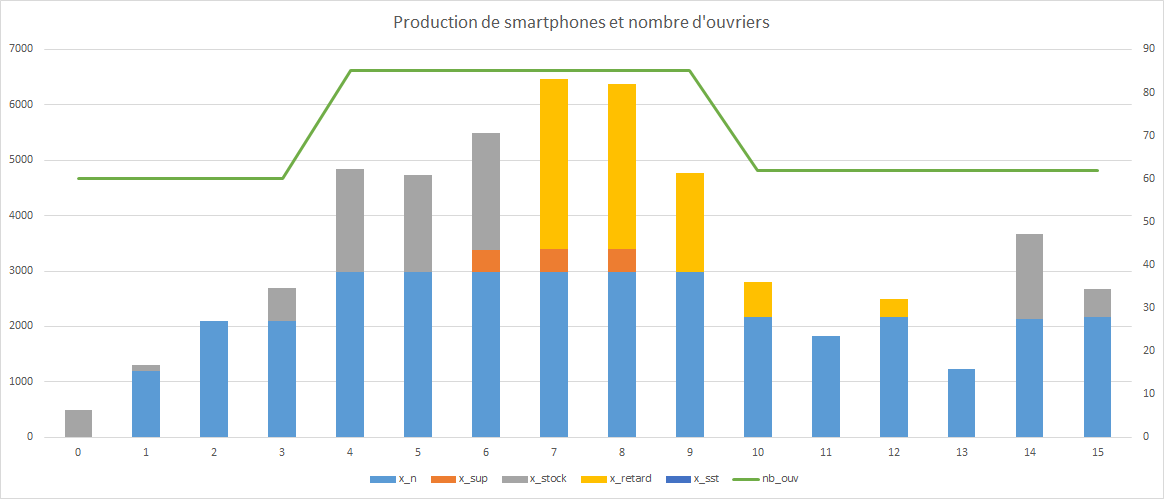
\includegraphics[scale = 0.8]{img/grapheProductionOuv.png}
	  \caption{Répartition du moyen de production des smartphones en fonction des semaines et évolution du nombre d'ouvriers dans le cas entier.}
	  \label{fig:grapheProductionOuv}
  \end{center}
\end{figure}
\question %10
\emph{Critiquez les modèles proposés dans ce projet. Sont-ils réalistes ?
Des approximations ont-elles été faites et, si oui sont-elles justifiées ?
Quelles améliorations pourriez-vous proposer (sans rentrer dans les détails),
avec quel impact potentiel sur la résolution du problème.}



\newpage

\appendix
\section{Utilisation de la fonction \texttt{kron}}
\label{app:kron}

\lstset{language=MATLAB}

Afin de comprendre l'utilité et l'efficacité de la fonction \texttt{kron},
voici son application pour la contrainte
\[ 
  \Delta\xstock + \texttts{demande}(s) = \xn + \xsup 
  + \xretard + \xsst - \myX{s-1}{retard} \qquad \forall s
\]
pour une planification sur deux semaines ($\texttt{d.T}=2$).

Voici le code correspondant
\begin{lstlisting}
  dSeg   = [1 1 -1 1 1];
  dpSeg  = [0 0 1 -1 0];
  Aeq = [kron([eye(d.T),zeros(d.T,1)],dpSeg) ...
       + kron([zeros(d.T,1),eye(d.T)],dSeg)];
  beq = [d.demande'];   
\end{lstlisting}

L'instruction \lstinline{kron(A,B)} effectue l'opération suivante
\[ 
  \texttts{kron}
    \left(
      \begin{pmatrix} a_{1,1} & a_{1,2} \\ a_{2,1} & a_{2,2} \end{pmatrix}, 
      \texttts{B}
    \right)
  =
  \begin{pmatrix} a_{1,1} \cdot\texttts{B} & a_{1,2} \cdot\texttts{B}
    \\ a_{2,1}\cdot\texttts{B} & a_{2,2} \cdot\texttts{B}
  \end{pmatrix}
\]

Nous avons donc tout d'abord la matrice créée à la ligne $3$
\[
    \left(
    \begin{array}{*{15}c}
      0 & 0 & 1 & -1 & 0 & 0 & 0 &  0 & 0 & 0 & 0 & 0 & 0 & 0 & 0 \\
      0 & 0 & 0 &  0 & 0 & 0 & 0 & -1 & 1 & 0 & 0 & 0 & 0 & 0 & 0 
    \end{array}
    \right),
\]

ensuite celle créée à la ligne $4$
\[
    \left(
    \begin{array}{*{15}c}
      0 & 0 & 0 & 0 & 0 & 1 & 1 & -1 & 1 & 1 & 0 & 0 & 0 & 0 & 0 \\
      0 & 0 & 0 & 0 & 0 & 0 & 0 &  0 & 0 & 0 & 1 & 1 & -1 & 1 & 1 
    \end{array}
    \right).
\]


Rappelons la forme de notre vecteur $x_s$
\[ x_s = 
  \begin{pmatrix} 
    \xn &\xsup &\xstock &\xretard &\xsst
  \end{pmatrix}^T.
\]

Cela donne comme voulu $A_{eq} \, x = b_{eq}$
\[
    \left(
    \begin{array}{*{15}c}
      0 & 0 & 1 & -1 & 0 & 1 & 1 & -1 & 1 & 1 & 0 & 0 &  0 & 0 & 0 \\
      0 & 0 & 0 &  0 & 0 & 0 & 0 & -1 & 1 & 0 & 1 & 1 & -1 & 1 & 1 
    \end{array}
    \right)
    \left(
    \begin{array}{*{1}l}
      \myX{0}{n}\\ \myX{0}{sup}\\ \myX{0}{stock}\\ \myX{0}{retard}\\ \myX{0}{sst}\\
      \myX{1}{n}\\ \myX{1}{sup}\\ \myX{1}{stock}\\ \myX{1}{retard}\\ \myX{1}{sst}\\
      \myX{2}{n}\\ \myX{2}{sup}\\ \myX{2}{stock}\\ \myX{2}{retard}\\ \myX{2}{sst}
    \end{array}
    \right)
    = 
    \left(
    \begin{array}{*{1}l}
      \texttts{demande}(1) \\ \texttts{demande}(2)
    \end{array}
    \right)
    \text.
\]

Cette méthode s'avère simple et efficace puisque ces $5$ lignes de code suffisent 
à remplir notre matrice peu importe le nombre de semaines.


\end{document}